Onderstaande funtie berekent de co\"effici\"entenmatrix $C \in \mathbb{R}^({n+1) \times (m+1)}$, gegeven de vectoren $x \in \mathbb{R}^{M}$ en $y \in \mathbb{R}^{N}$ als 2D meetpunten, de matrix $F \in \mathbb{R}^{N \times M}$ met functie- of meetwaarden en de parameters $m,n \in \mathbb{N}$ die respectievelijk de graad in $x$ en $y$ van de benaderende veeltermen.
\lstinputlisting[
  style      = Matlab-editor,
  basicstyle = \mlttfamily,
]{kkb.m}

Er werd een kleine test op deze functie uitgevoerd. Hierbij is de input: $x = \begin{bmatrix}1&2&3\end{bmatrix}, y = \begin{bmatrix}1&2&3\end{bmatrix}, m = 3, n = 2$ en
$$F = \begin{bmatrix}1&2&1\\
2&3&2\\
1&2&1\end{bmatrix}.$$
De punten werden samen geplot met het benaderend oppervlak in figuur \ref{fig:oef11}.

\begin{figure}[htb]
    \centering
    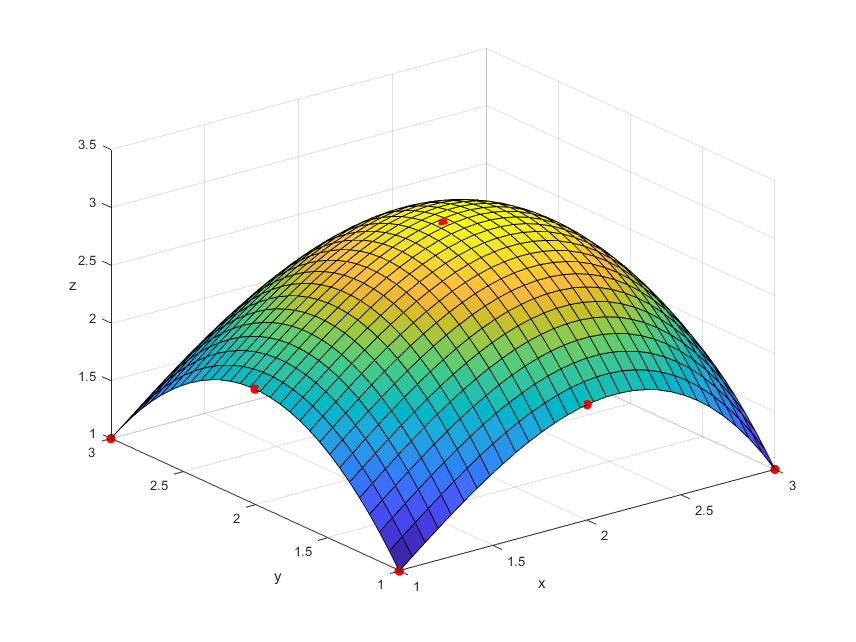
\includegraphics[width=0.7\textwidth]{oef11.png}
    \caption{test van het kkb algoritme}
    \label{fig:oef11}
\end{figure}